\documentclass[10pt,a4paper]{article}
\usepackage[utf8]{inputenc}
\usepackage[T1]{fontenc}
\usepackage[spanish,es-tabla]{babel}
\usepackage{mathptmx}                       % Times
\usepackage[a4paper,margin=1.8cm,columnsep=0.7cm]{geometry}
\usepackage{microtype,graphicx,booktabs,tabularx,array,amsmath,enumitem,titlesec}
\usepackage[font=footnotesize,labelfont=bf,skip=2pt]{caption}
\usepackage[hyphens]{url}
\usepackage[hidelinks]{hyperref}

% ---- Compactación tipográfica (cuerpo <= 2 páginas) ----
\setlength{\parindent}{1em}
\setlength{\parskip}{0pt}
\linespread{0.97}
\setlist{nosep,leftmargin=1.1em,topsep=1pt}
\titleformat{\section}{\normalfont\bfseries\normalsize}{\thesection.}{0.4em}{}
\titlespacing*{\section}{0pt}{5pt}{2pt}
\renewcommand{\arraystretch}{1.05}
\setlength{\textfloatsep}{5pt plus 1pt minus 1pt}
\setlength{\intextsep}{4pt}
\setlength{\tabcolsep}{3pt}
\newcommand{\nota}{$^{\dagger}$}

\begin{document}

% ======================= PÁGINA 1: CARÁTULA =======================
\thispagestyle{empty}
\begin{center}
\vspace*{1.5cm}
{\Large\bfseries Universidad Técnica Estatal de Quevedo (UTEQ)}\\[6pt]
{\large Facultad de Ciencias de la Ingeniería --- Computación}\\[3.5cm]
{\large\textbf{Asignatura:} Sistemas Distribuidos}\\[4pt]
{\large\textbf{Código de actividad:} FORM-AC-01 \quad|\quad \textbf{Grupo 3}}\\[2.5cm]
{\LARGE\bfseries Análisis de caso: Fallo masivo en la infraestructura distribuida de Meta (Facebook) --- 4 de octubre de 2021}\\[3cm]
{\large\textbf{Integrantes del equipo}}\\[8pt]
{\large
ESPAÑA VERA KENNY ISAIAS\\
JARAMILLO ACOSTA LUIS JEREMY\\
PACA PILATAZA LUIS ALBERTO\\
ZAMBRANO RONQUILLO HEINER ARIEL}\\[3cm]
{\large\textbf{Fecha:} 14 de noviembre de 2026}
\end{center}
\newpage

% =================== PÁGINAS 2 Y 3: DESARROLLO TÉCNICO ===================
\twocolumn
\begin{figure*}[t]
\centering
\IfFileExists{arbol_fallos_facebook2021.pdf}{%
  \includegraphics[width=\textwidth,height=11cm,keepaspectratio]{arbol_fallos_facebook2021.pdf}}{%
\IfFileExists{arbol_fallos_facebook2021.png}{%
  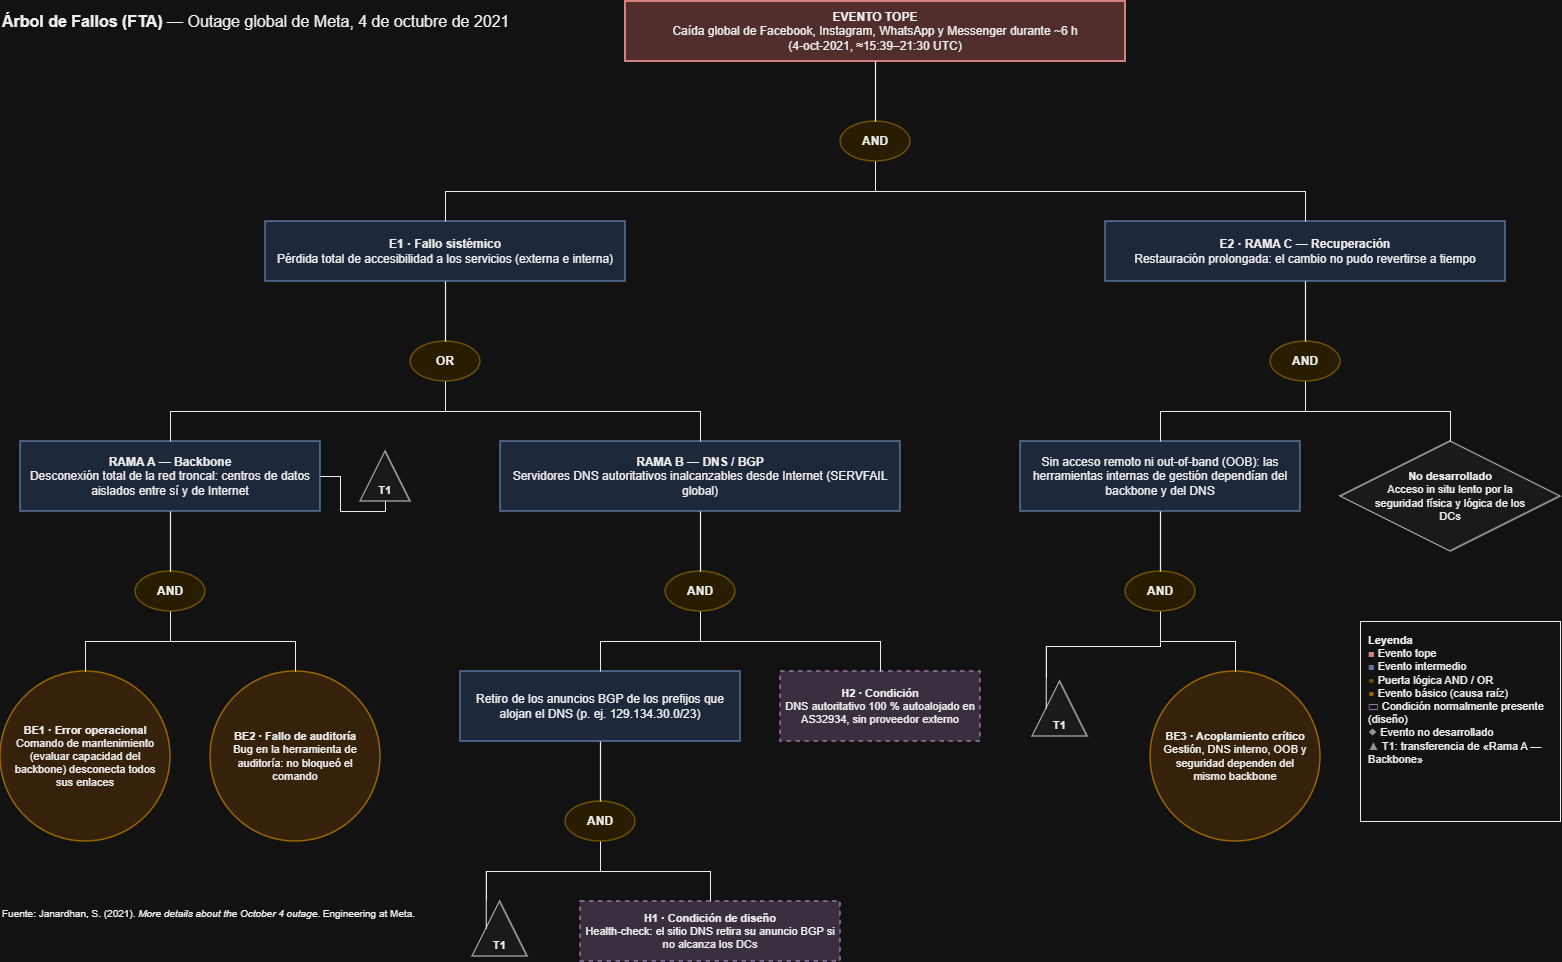
\includegraphics[width=\textwidth,height=11cm,keepaspectratio]{arbol_fallos_facebook2021.png}}{%
  \fbox{\parbox[c][10cm][c]{0.9\textwidth}{\centering\ttfamily [PLACEHOLDER] Exportar el .drawio como PDF y guardarlo como arbol\_fallos\_facebook2021.pdf junto a este .tex}}}}
\caption{Árbol de Fallos (FTA) del \textit{outage} de Meta del 4 de octubre de 2021. Elaboración propia a partir de~\cite{janardhan2021outage}.}\label{fig:fta}
\end{figure*}

%%%%%%%%%%%%%%%%%%%% FASE 1: Incidente y línea de tiempo %%%%%%%%%%%%%%%%%%%%
\section{Descripción del incidente y línea de tiempo}
El 4 de octubre de 2021, Facebook, Instagram, WhatsApp, Messenger y Oculus, junto con las herramientas internas de Meta, quedaron inaccesibles a escala global durante $\approx$6\,h (de $\approx$15:40 a $\approx$21:30 UTC; 10:40--16:30 en Ecuador, UTC$-5$). Meta lo atribuyó a un cambio de configuración defectuoso en los enrutadores de su red troncal, sin actividad maliciosa ni evidencia de compromiso de datos~\cite{janardhan2021update}; su análisis posterior detalló la cadena de causas~\cite{janardhan2021outage}. La Tabla~\ref{tab:linea} resume la cronología medida externamente por Cloudflare~\cite{cloudflare2021facebook}.

\begin{table}[h]
\centering\footnotesize
\caption{Línea de tiempo del incidente (UTC).}\label{tab:linea}
\begin{tabularx}{\columnwidth}{@{}l X@{}}
\toprule
\textbf{Hora} & \textbf{Evento}\\\midrule
15:40 & Pico de actualizaciones BGP de Facebook: se retiran las rutas hacia los prefijos de sus DNS autoritativos~\cite{cloudflare2021facebook}.\\
15:50 & \texttt{facebook.com} deja de resolverse en 1.1.1.1 (SERVFAIL).\\
15:58 & Cloudflare confirma que Facebook dejó de anunciar rutas a sus prefijos DNS.\\
Durante la caída & Sin acceso remoto ni \textit{out-of-band}; el equipo debe acudir a los centros de datos~\cite{janardhan2021outage}.\\
$\approx$21:00 & Reaparece actividad BGP de Facebook (pico a las 21:17).\\
21:20 & \texttt{facebook.com} vuelve a resolverse en 1.1.1.1.\\
21:28 & Facebook reconectado a Internet; DNS operativo. Siguió una reposición gradual de la carga.\\
\bottomrule
\end{tabularx}
\end{table}

%%%%%%%%%%%%%%%%%%%% FASE 2: Causas raíz e impacto %%%%%%%%%%%%%%%%%%%%
\section{Análisis de causas raíz}
El Árbol de Fallos (Fig.~\ref{fig:fta}) se lee de arriba abajo: el evento tope (caída global de $\approx$6\,h) exige que coincidan un fallo sistémico (E1) y una recuperación prolongada (E2).

\paragraph{Rama A: backbone.} En un mantenimiento rutinario, un comando pensado para evaluar la capacidad de la red troncal desconectó todos sus enlaces (BE1); la herramienta de auditoría, que normalmente bloquea comandos así, tenía un \textit{bug} que impidió detenerlo (BE2)~\cite{janardhan2021outage}.

\paragraph{Rama B: DNS/BGP.} Sin backbone, los sitios DNS no alcanzaban los centros de datos y, por diseño (H1), retiraron sus anuncios BGP: los servidores seguían encendidos pero inalcanzables. Como el DNS autoritativo estaba íntegramente en el AS32934 de Facebook (H2), Internet no pudo resolver sus dominios~\cite{janardhan2021outage,cloudflare2021facebook}. Los reintentos de los resolvers multiplicaron la carga: 1.1.1.1 recibió 30$\times$ más consultas~\cite{cloudflare2021facebook} y el tráfico hacia servidores \texttt{.COM/.NET} pasó de $\approx$7\,000 a $\approx$900\,000 consultas/s~\cite{rfc9520}.

\paragraph{Rama C: recuperación.} Las herramientas de gestión, el DNS interno y el acceso OOB dependían del mismo backbone (BE3), así que nadie pudo revertir el cambio en remoto; el acceso físico fue lento por las medidas de seguridad~\cite{janardhan2021outage}. Un error puntual se convirtió en $\approx$6\,h de caída.

Es un fallo de modo común: una redundancia aparente (varios sitios DNS) compartía un mismo dominio de fallo. La concentración de la infraestructura DNS se ha medido empíricamente~\cite{xu2023centrality}, y estudios recientes sobre la fragilidad de las redes IP~\cite{owen2025failures}, los fallos en cascada~\cite{zheng2026tolerance} y la detección de anomalías BGP~\cite{wu2025glbad,latifmartinez2025bgp} tratan incidentes de este tipo.

\section{Impacto cuantificado}
\begin{table}[h]
\centering\footnotesize
\caption{Impacto del incidente.}\label{tab:impacto}
\begin{tabularx}{\columnwidth}{@{}l X@{}}
\toprule
\textbf{Indicador} & \textbf{Valor}\\\midrule
Usuarios en riesgo & $\approx$3\,500 millones de usuarios de las plataformas de Meta\nota\\
Indisponibilidad del DNS & $\approx$5\,h 48\,min (15:40--21:28 UTC)~\cite{cloudflare2021facebook}\\
Ingresos publicitarios & $\approx$USD 545\,000/h solo en EE.\,UU.\nota; $\approx$USD 100\,M globales (estimación: ingreso medio por hora $\times$ duración)\nota\\
Bolsa & Acción $-4{,}9\,\%$ el 4-oct\nota; coincidió con otras noticias adversas, no es atribuible solo a la caída\\
Disponibilidad mensual & $1-5{,}8/720\approx 99{,}19\,\%$ (cálculo propio)\\
\bottomrule
\end{tabularx}
{\scriptsize\nota\ Cifras de prensa económica (Reuters, Fortune); no forman parte de las referencias académicas verificadas.}
\end{table}
Las fuentes verificadas no mencionan un SLA contractual. Como referencia usamos el 99,5\,\% de nuestro PFC (presupuesto de 3,6\,h/mes): un 99,19\,\% lo incumple.

%%%%%%%%%%%%%%%%%%%% FASE 3: Unidad 1 y mitigación %%%%%%%%%%%%%%%%%%%%
\section{Relación con la Unidad 1}
\paragraph{Transparencia de distribución.} Se rompió la de \textit{acceso} (los clientes no pudieron resolver nombres), la de \textit{ubicación} (DNS/BGP es el mecanismo que mapea nombre a dirección alcanzable) y la de \textit{fallos}: las réplicas seguían vivas pero la falla no se enmascaró, y ni siquiera los empleados pudieron alcanzarlas.

\paragraph{Teorema CAP (analogía).} La retirada de BGP produjo una partición total ($P$) entre los clientes y los centros de datos. Ante $P$ hay que elegir: Meta quedó sin disponibilidad ($A$) y sin consistencia observable ($C$), porque ninguna lectura ni escritura llegó a servirse. Internamente, los planos de control quedaron aislados del backbone y entre sí. CAP se refiere a datos replicados, por lo que aquí es solo una analogía.

\paragraph{Mecanismo de tolerancia que falló.} El \textit{health-check} que retira el anuncio BGP al perder los centros de datos sirve ante un fallo parcial, pero con el backbone caído declaró ``enfermos'' a todos los sitios DNS a la vez~\cite{janardhan2021outage}. Faltaron aislamiento de fallos (\textit{bulkheads}) y un acceso OOB independiente de la red que se intenta reparar.

\section{Mitigación aplicada}
\begin{table}[h]
\centering\footnotesize
\caption{Medidas inmediatas y estructurales.}\label{tab:mitiga}
\begin{tabularx}{\columnwidth}{@{}l X@{}}
\toprule
\textbf{Tipo} & \textbf{Medida}\\\midrule
Inmediata & Acceso físico de emergencia a los centros de datos y restauración manual del backbone~\cite{janardhan2021outage}.\\
Inmediata & Reposición gradual de carga, BGP y DNS para evitar picos de tráfico y de consumo eléctrico (decenas de MW), apoyada en los simulacros \textit{storm}~\cite{janardhan2021outage}.\\
Estructural (declarada) & Revisión amplia de resiliencia, nuevos escenarios de \textit{storm} que simulen la caída global del backbone y más pruebas~\cite{janardhan2021outage}.\\
Estructural (propuesta del equipo) & Auditor/simulador de comandos de red con validación independiente, herramientas internas desacopladas del backbone y acceso OOB resiliente. Meta no los confirma en sus publicaciones.\\
\bottomrule
\end{tabularx}
\end{table}

% ======================= PÁGINA 4: REFERENCIAS =======================
\newpage
\onecolumn
\small
\bibliographystyle{IEEEtran}
\bibliography{referencias}

\end{document}
